%%% Local Variables:
%%% mode: latex
%%% TeX-master: "../doc"
%%% coding: utf-8
%%% End:
% !TEX TS-program = pdflatexmk
% !TEX encoding = UTF-8 Unicode
% !TEX root = ../doc.tex
\section{Einführung}
Als Level Of Detail (LOD) werden die verschiedenen Detailstufen bei der virtuellen Darstellung bezeichnet.
Dies wird verwendet, um die Geschwindigkeit von Anwendungen zu steigern, indem Objekte im Nahbereich detailiert angezeigt werden; wohingegen Elemente im Fernbereich deutlich vereinfacht dargestellt werden.

\subsection{Das Problem}
Geometrische Objekte können zu Komplex werden, um jederzeit performant und interaktiv gerendert zu werden.
Gerade wenn viele Objekte zur selben Zeit sichtbar sind, lohnt es sich, zu priorisieren und gewisse Objekte in reduzierter Qualität anzuzeigen.
Im Idealfall geschieht dies jedoch, ohne dass der Anwender dies bemerkt.

\subsection{Lösungsansätze}
In diesem Abschnitt werden mögliche Ansätze erklärt, welche helfen sollen, die Render-Perfomanz zu erhöhen. Diese Arbeit konzentriert sich jedoch auf den Ansatz von Level of Detail; die anderen Ansätze werden nur kurz erläutert.

\paragraph{Level of Detail}
Level of Detail auch bekannt als polygonale Simplifizierung, geometrische Simplifizierung oder Mesh Reduzierung basiert darauf, die Komplexität von Objekten zu reduzieren, welche weiter von der Kamera entfernt werden. Es gibt verschiedene Ansätze zur Generierung von LODs, welche in Abschnitt XY im Detail erläutert werden. Zudem braucht es einen berechenbare Methode, die Genauigkeit von Modellen zu definieren, um diese entsprechend anzuwenden. Schlussendlich ist dann noch zu definieren, ab wann welche Artefakte verwendet werden soll, basierend auf der Genauigkeit und der Komplexität.

\begin{figure}[H]
\centering
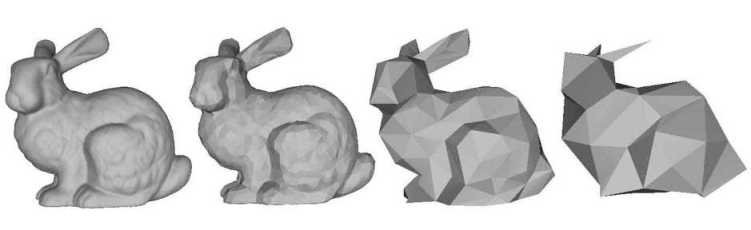
\includegraphics[width=0.8\columnwidth]{LODs-of-a-bunny-model-Courtesy-Stanford-3D-Scanning-Repository-From-left-to-right}
\caption{Level Of Detail Visualisierung vier Hasen}
\label{fig:LevelOfDetailVisualisierungvierHasen}
\end{figure}

Wie in der Abbildung \ref{fig:LevelOfDetailVisualisierungvierHasen} zu erkennen ist, wird von links nach rechts der Detailgrad und somit die Komplexität des Objektes reduziert. Sind es im Bild ganz links noch 69'451 Polygone, wird es bereits im ersten Schritt auf 2'502 Polygone reduziert. Dies ist eine enorme Reduktion von ca 96.5\%. Im dritten Schritt wird die Anzahl Polygone wiederum um ca. 90\% auf 251 reduziert. Schlussendlich hat das letzte Objekt noch 76 Polygone was knapp 0.1\% der ursprünglichen Anzahl entspricht.

\paragraph{Parallel rendering}
Lorem ipsum

\paragraph{Frustum culling}
Polygone, welche nicht im Kamera Frustum enthalten sind, werden bei dieser Methode nicht weiter prozessiert.
Dies reduziert die Anzahl Polygone drastisch.

\paragraph{Occlusion culling}
Polygone bzw. Objekte, welche komplett von anderen Objekten überdeckt werden, werden bei dieser Variante nicht prozessiert.

\paragraph{Backface culling}
Bei dieser Methode wird berechnet welche Polygone zur Kamera orientiert sind.
Alle Polygone, welche in die andere Richtung zeigen werden nicht gezeichnet.
Dies ist nicht immer gewünscht, für die meisten Anwendungen ist diese Optimierung jedoch aktiviert.

\paragraph{Image-based rendering}
Lorem ipsum


\subsection{Verschiedene Ansätze zur Generierung von LOD Modellen}
Es gibt verschiedene Ansätze, 3D-Modelle mittels LOD zu vereinfachen. In diesem Abschnitt werden einige davon detaillierter erläutert so wie ihre Vor- und Nachteile aufgezeigt.

\paragraph{Diskrete LOD (DLOD)}
Bei diskreten LOD werden für ein detailliertes Modell mehrere weniger detaillierte Modelle verwendet.
Abhängig von der Distanz zum Betrachter wird das optimale Modell gewählt.
\begin{itemize}
  \pro Simplizität: Keine Anpassungen am Scene Graph notwendig
  \con Harte Grenzen: Veränderung des Objektes kann merkbar sein
  \con Kein Clustering möglich: Probleme bei sehr grossen oder vielen kleinen Modellen
\end{itemize}

\paragraph{Kontinuierliche LOD (CLOD)}
Im Gegensatz zu DLOD wird bei CLOD vereinfachende Veränderungen an einem Modell gespeichert.
\begin{itemize}
  \pro Weiche Grenzen: Interpolation zwischen Auflösungen ist möglich
  \con Runtime Performance
  \con Kein Clustering möglich
\end{itemize}

\paragraph{Hierarchische LOD (HLOD)}
Bei HLOD werden mehrere Objekte in einen Cluster gruppiert.
\begin{itemize}
  \pro Clustering möglich
\end{itemize}
